%
\section{Demo}%
%
\edef\maxSat{MAX-SAT}%
\edef\maxTSat{MAX-3SAT}%
\def\oFlip{\ensuremath{1}-flip}%
\def\tFlip{\ensuremath{2}-flip}%
\def\mFlip{\ensuremath{m}-flip}%
%
\gdef\maxSatClauses{\textcolor{blue}{\ensuremath{k}}}%
\gdef\maxSatVariables{\textcolor{green}{\ensuremath{n}}}%
\gdef\maxSatVariable{\ensuremath{x}}%
\gdef\maxSatVariablei#1{\ensuremath{\maxSatVariable_{#1}}}%
\gdef\maxSatFormula{\ensuremath{B}}%
%
\begin{frame}[t]%
\frametitle{\maxSat}%
\begin{itemize}%
\item \only<8->{Maximum }Satisfiability Problems (SAT)\only<-7>{\scitep{HS2000SAORFROS}}\only<8->{\scitep{HS2005SLSFAA}}\uncover<2->{:%
\begin{itemize}
\item Given: Formula \maxSatFormula\ in Boolean logic%
\uncover<3->{ with of \maxSatVariables\ Boolean variables $\vec{\maxSatVariable}=(\maxSatVariablei{1}, \maxSatVariablei{2},\dots, \maxSatVariablei{\maxSatVariables})$%
\uncover<4->{, which appear either directly or negated%
\uncover<5->{ in \maxSatClauses\ \inQuotes{\texttt{or}} clauses%
\uncover<6->{, which are all combined with into one \inQuotes{\texttt{and}}}}}}%
\item<7-> \only<-7>{SAT Goal: find a setting for these variables so that $\maxSatFormula$ becomes \texttt{true}}%
\only<8->{\maxSat\ Goal\scitep{HS2005SLSFAA}: minimize objective function $\objectiveFunctionb{\vec{x}} = \textnormal{number of clauses which are \texttt{false}}$.}%
\item<9-> $\objectiveFunctionb{\vec{x}}=0$ $\Longrightarrow$ all clauses are \texttt{true}, SAT problem solved%
\end{itemize}%
}%
%
\item<10-> We want to compare the performance of \textcolor{red}{six different} (trivial) \textcolor{red}{algorithm setups}\uncover<11->{:%
\begin{enumerate}%
\item 1-flip Hill Climber%
\item 1-flip Hill Climber with Restarts%
\item 2-flip Hill Climber%
\item 2-flip Hill Climber with Restarts%
\item $m$-flip Hill Climber%
\item $m$-flip Hill Climber with Restarts%
\end{enumerate}%
}%
%
\item<12-> For the experiment, we want to solve $10\times 10$ (simple) instances from \satLib\expandafter\scitep{\satLibReferences} with \textcolor{red}{10 different values of \maxSatVariables} (and \maxSatClauses)%
%
\end{itemize}%
%
\locateGraphic{-2,7-9}{width=0.55\paperwidth}{graphics/problem_examples/sat/sat}{0.225}{0.54}%
\locateGraphic{3}{width=0.55\paperwidth}{graphics/problem_examples/sat/sat_variables}{0.225}{0.54}%
\locateGraphic{4}{width=0.55\paperwidth}{graphics/problem_examples/sat/sat_negation}{0.225}{0.54}%
\locateGraphic{5}{width=0.55\paperwidth}{graphics/problem_examples/sat/sat_or}{0.225}{0.54}%
\locateGraphic{6}{width=0.55\paperwidth}{graphics/problem_examples/sat/sat_and}{0.225}{0.54}%
%
\strut\\\strut\\\strut\\\strut\\\strut\\\strut\\\strut\\\strut%
%
\end{frame}%
%
%
\begin{frame}[t]%
\frametitle{Installation}%
\centering\footnotesize%
%
\strut\vfill%
\mbox{\textbf{\large{Website:~\href{http://optimizationbenchmarking.github.io}{http://optimizationbenchmarking.github.io}}}}%
\vfill%
%
\begin{itemize}%
%
\item \alert{Stand-Alone GUI}: easily store, annotate, and process your experimental results:%
\begin{itemize}%
\item client/server application: computation at the server, joint repository for data of your group%
\item software requirements: Java~7~JDK\scitep{JAVA2PSESAS}, TeX~Live\scitep{TEXLIVE}, \codeil{R}\scitep{WU2006TRPFSC} with several packages%
\item download software from web page%
\item \mbox{\codeil{java -jar evaluatorGui.jar}}%
\item open browser to \codeil{http://localhost:8080}%
\end{itemize}%
%
\uncover<2->{%
\vfill\vfill%
%
\item \alert{Application Dockerized for you!}%
\begin{itemize}%
\item install Docker from\\\url{http://www.docker.com/} and do%
\item \mbox{\codeil{docker run -t -i -p 9999:8080/tcp}} \mbox{\codeil{optimizationbenchmarking/evaluator-gui}}%
\item open browser to \codeil{http://localhost:9999} on Linux, replace \codeil{localhost} with the IP address of the Docker container under Windows or Mac OS%
\end{itemize}%
%
\vfill%
}%
%
\locateGraphic{2-}{width=0.33\paperwidth}{graphics/website/website}{0.63}{0.45}%
\locateGraphic{1}{width=0.33\paperwidth}{graphics/barcodes/website}{0.63}{0.47}%
%
\end{itemize}%
%
\end{frame}%
%

%
%
\begin{frame}[b,label=maxSatInteractiveDemoEnd]%
\frametitle{The Flow / Demo}%
%
\only<-1>{%
\strut\vfill\strut%
\centering{\LARGE{\textbf{\alert{The evaluator works as follows\dots}}}}%
\strut\vfill\strut%
}\only<2->{%
\strut\\\strut\\\strut\\\strut\\\strut\\\strut\\\strut\\\strut%
}%
%
\locate{2-3}{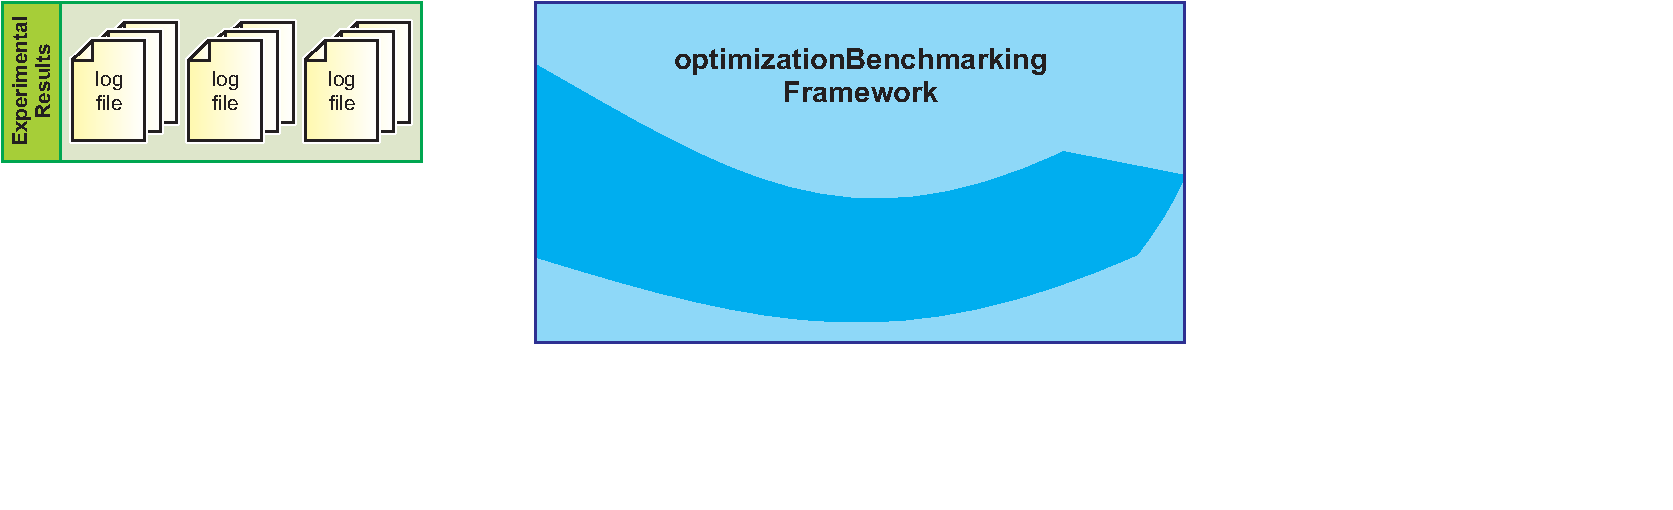
\includegraphics[width=0.9\paperwidth]{graphics/flow/flow_input_1_results}}{0.05}{0.16}%
\locate{4-5}{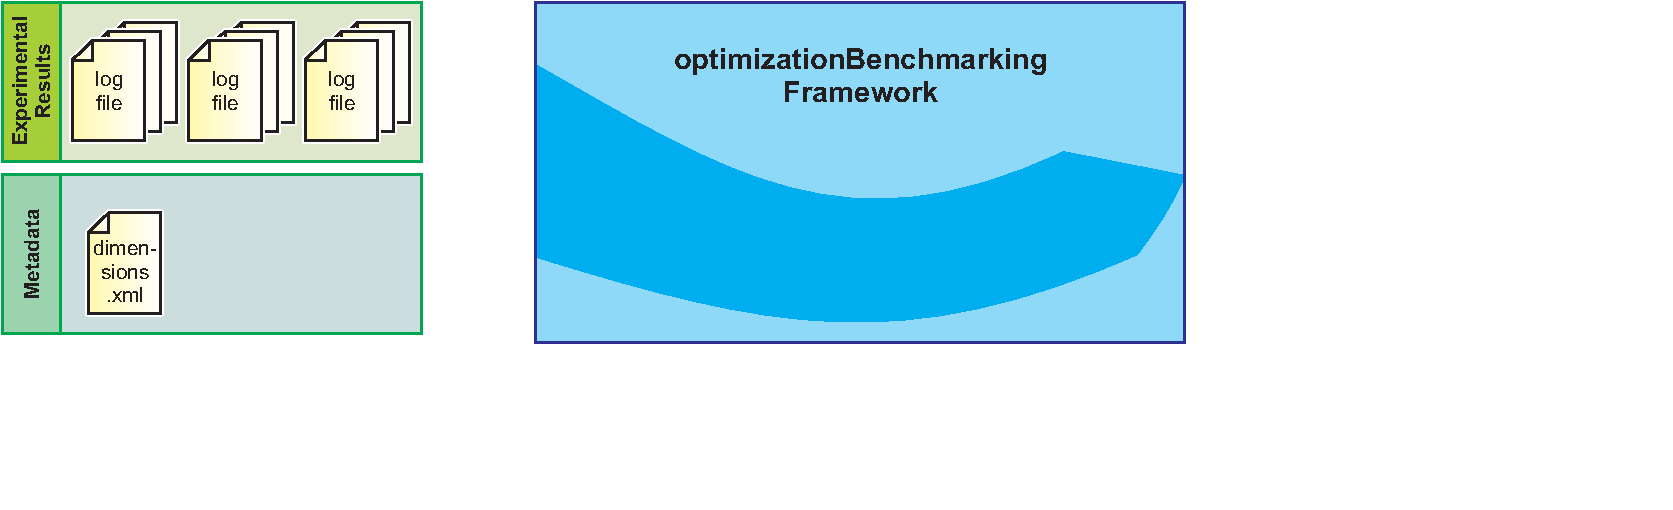
\includegraphics[width=0.9\paperwidth]{graphics/flow/flow_input_2_dimensions}}{0.05}{0.16}%
\locate{6-7}{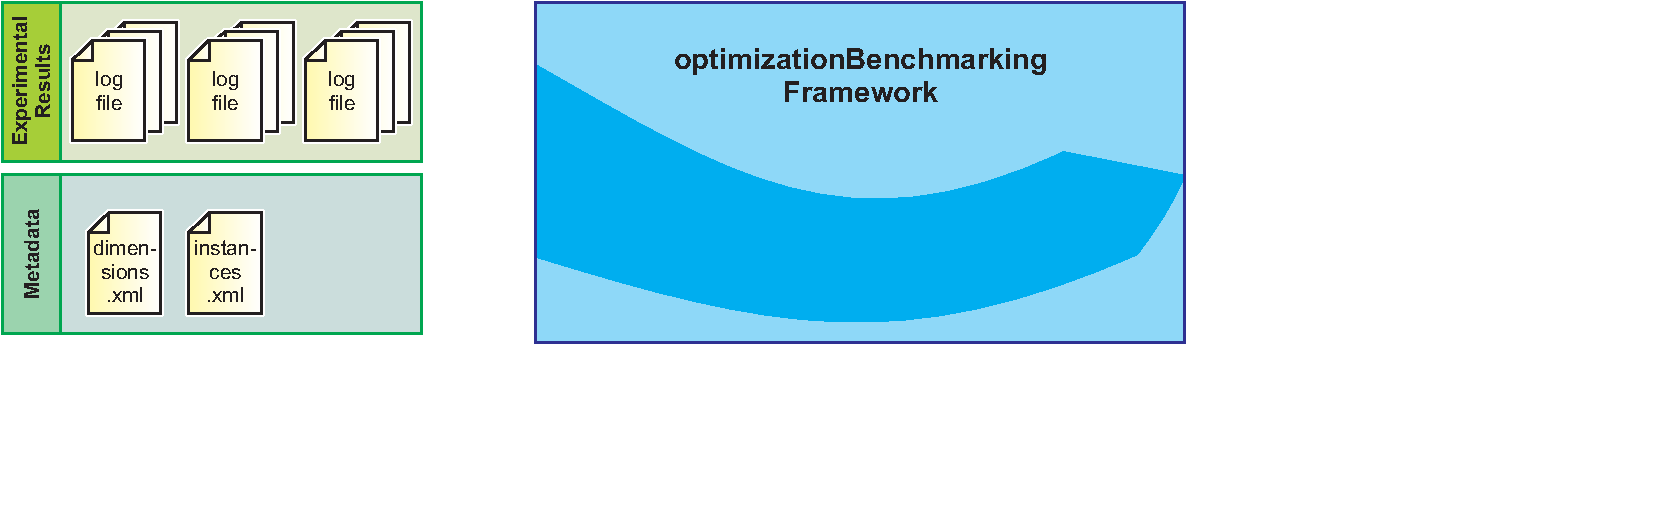
\includegraphics[width=0.9\paperwidth]{graphics/flow/flow_input_3_instances}}{0.05}{0.16}%
\locate{8-9}{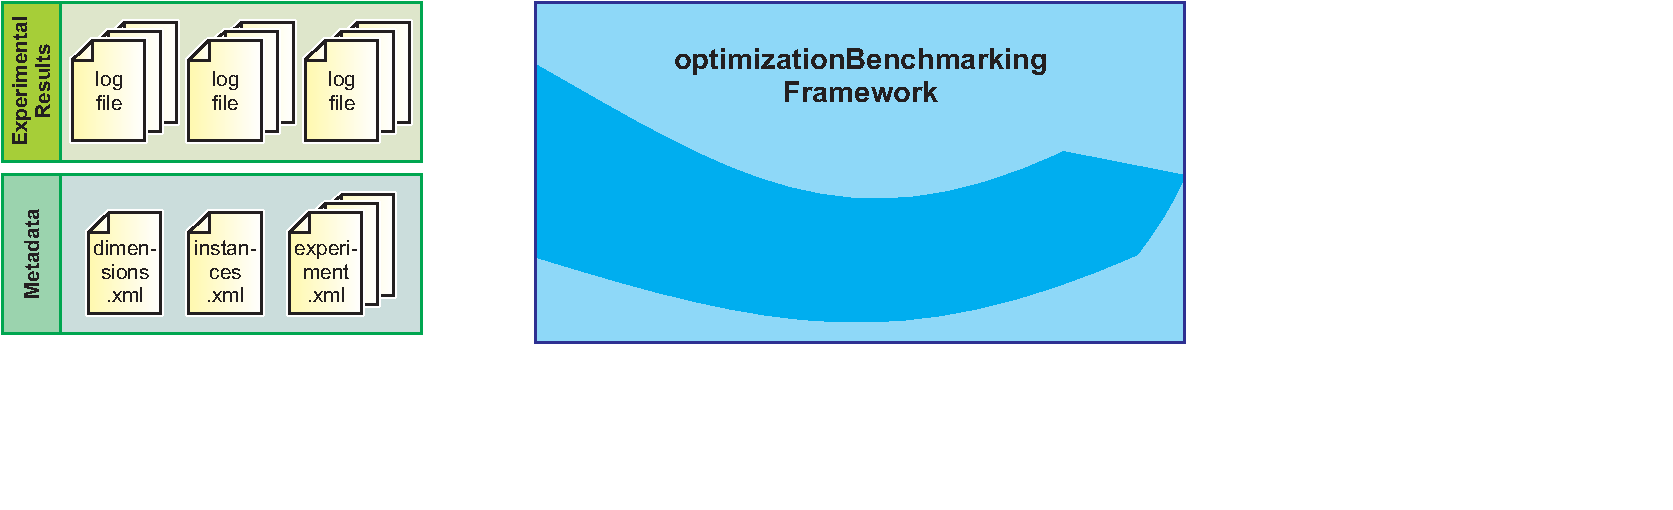
\includegraphics[width=0.9\paperwidth]{graphics/flow/flow_input_4_experiment}}{0.05}{0.16}%
\locate{10-11}{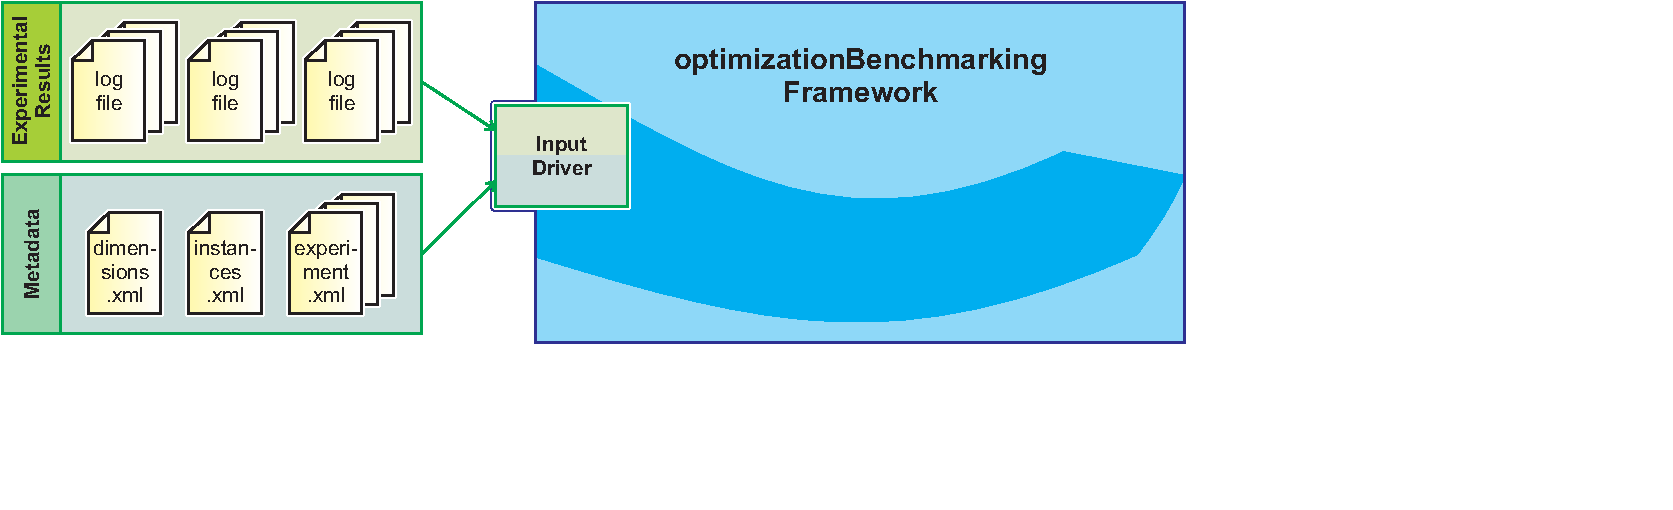
\includegraphics[width=0.9\paperwidth]{graphics/flow/flow_input_5_driver}}{0.05}{0.16}%
\locate{12}{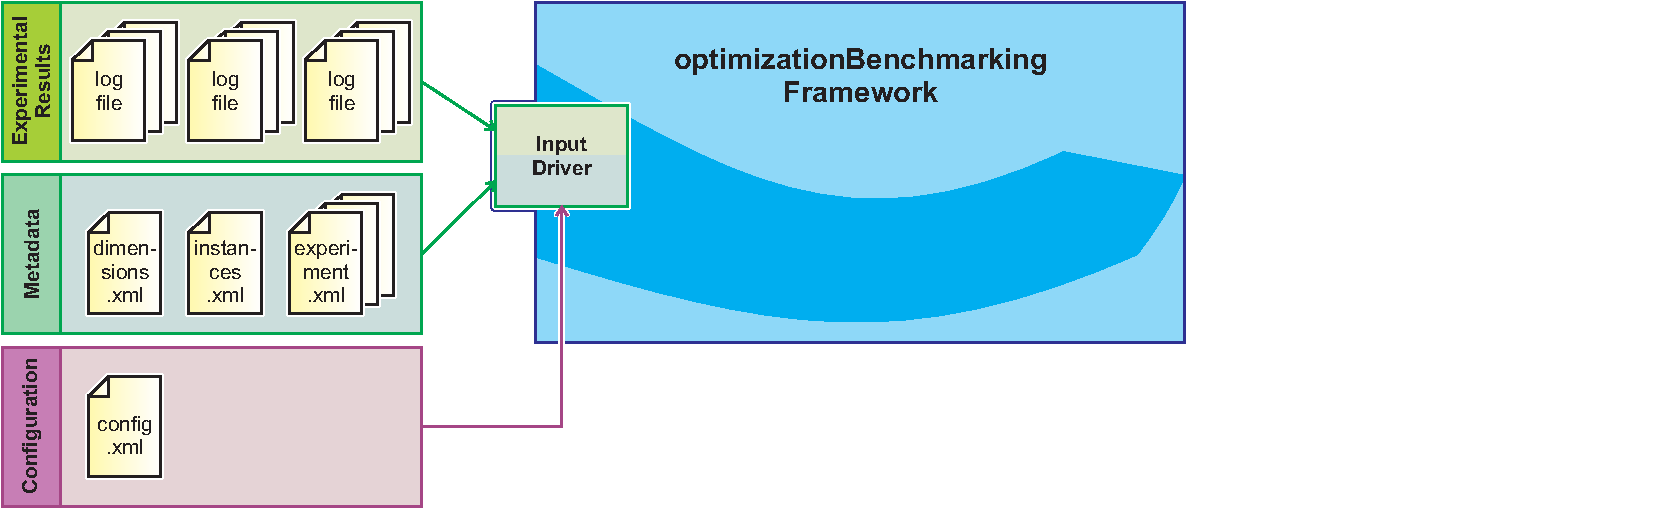
\includegraphics[width=0.9\paperwidth]{graphics/flow/flow_config_1_config}}{0.05}{0.16}%
\locate{13}{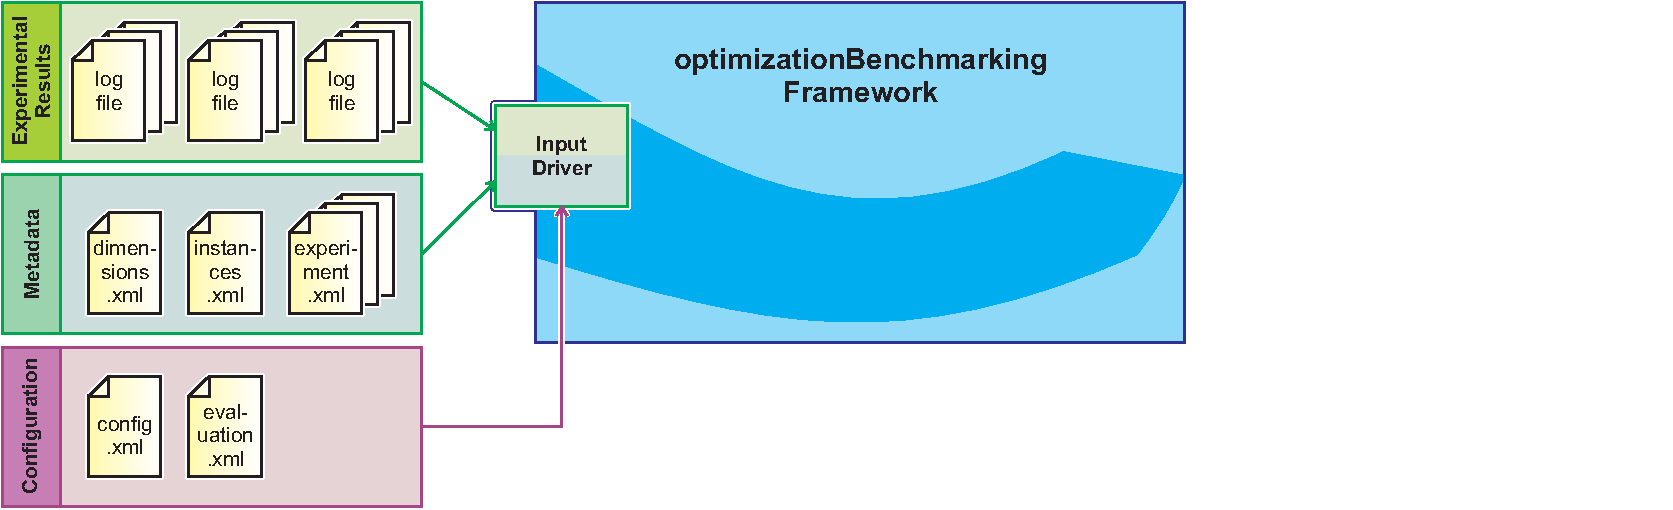
\includegraphics[width=0.9\paperwidth]{graphics/flow/flow_config_2_evaluation}}{0.05}{0.16}%
\locate{14-15}{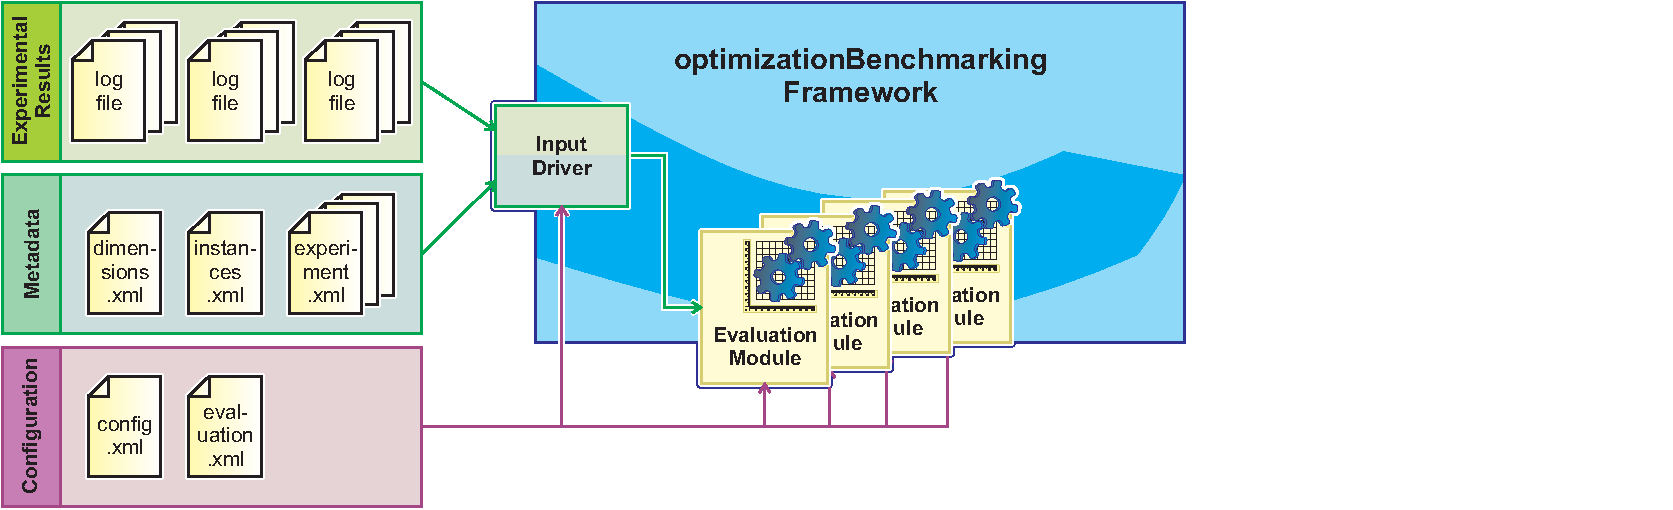
\includegraphics[width=0.9\paperwidth]{graphics/flow/flow_evaluation}}{0.05}{0.16}%
\locate{16}{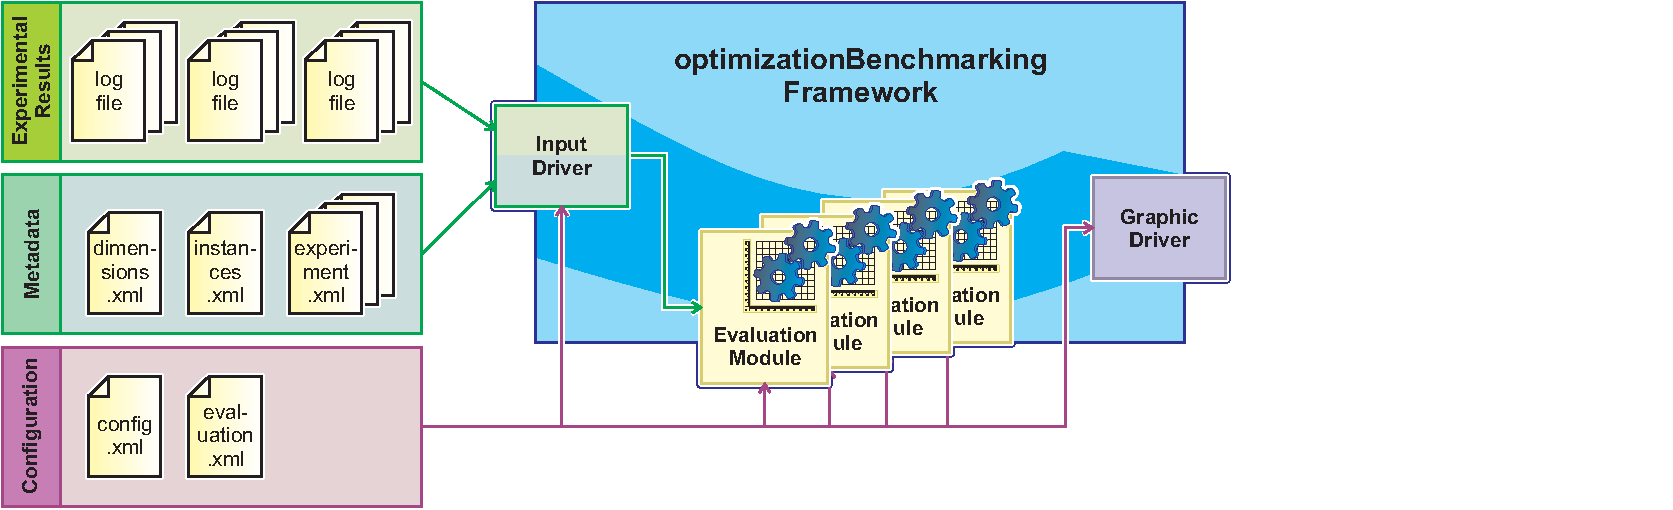
\includegraphics[width=0.9\paperwidth]{graphics/flow/flow_output_1_graphic}}{0.05}{0.16}%
\locate{17}{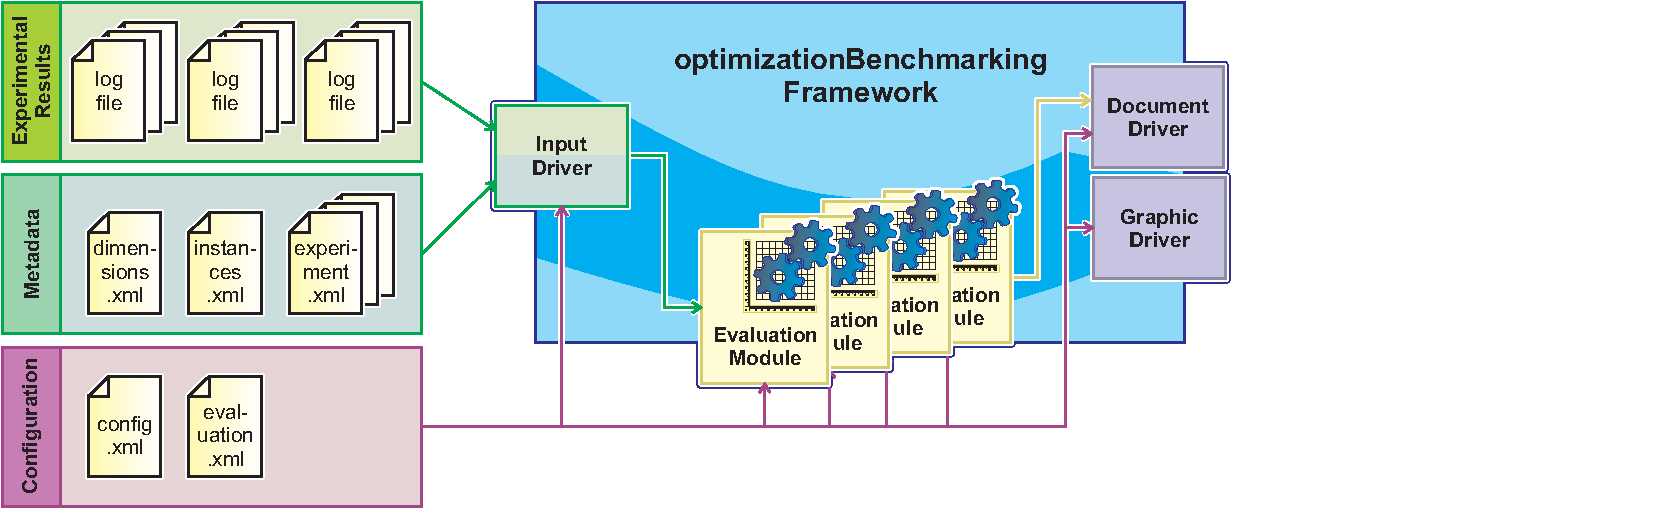
\includegraphics[width=0.9\paperwidth]{graphics/flow/flow_output_2_document}}{0.05}{0.16}%
\locate{18}{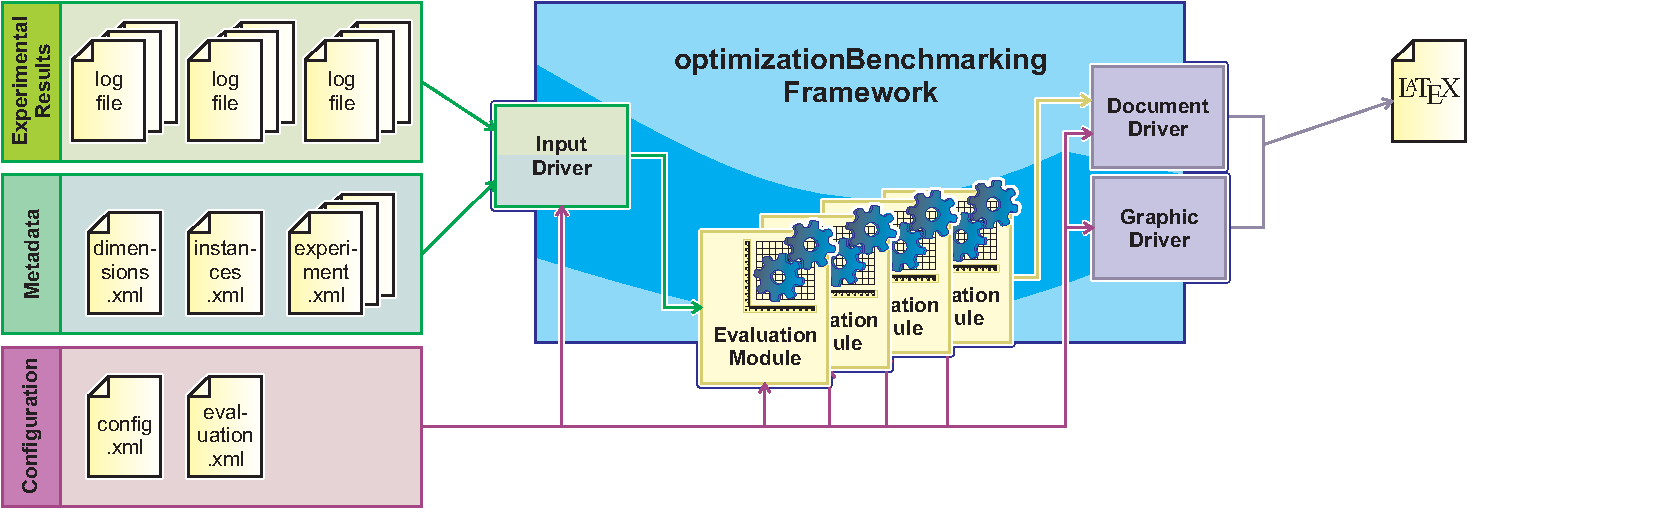
\includegraphics[width=0.9\paperwidth]{graphics/flow/flow_output_3_latex}}{0.05}{0.16}%
\locate{19-21}{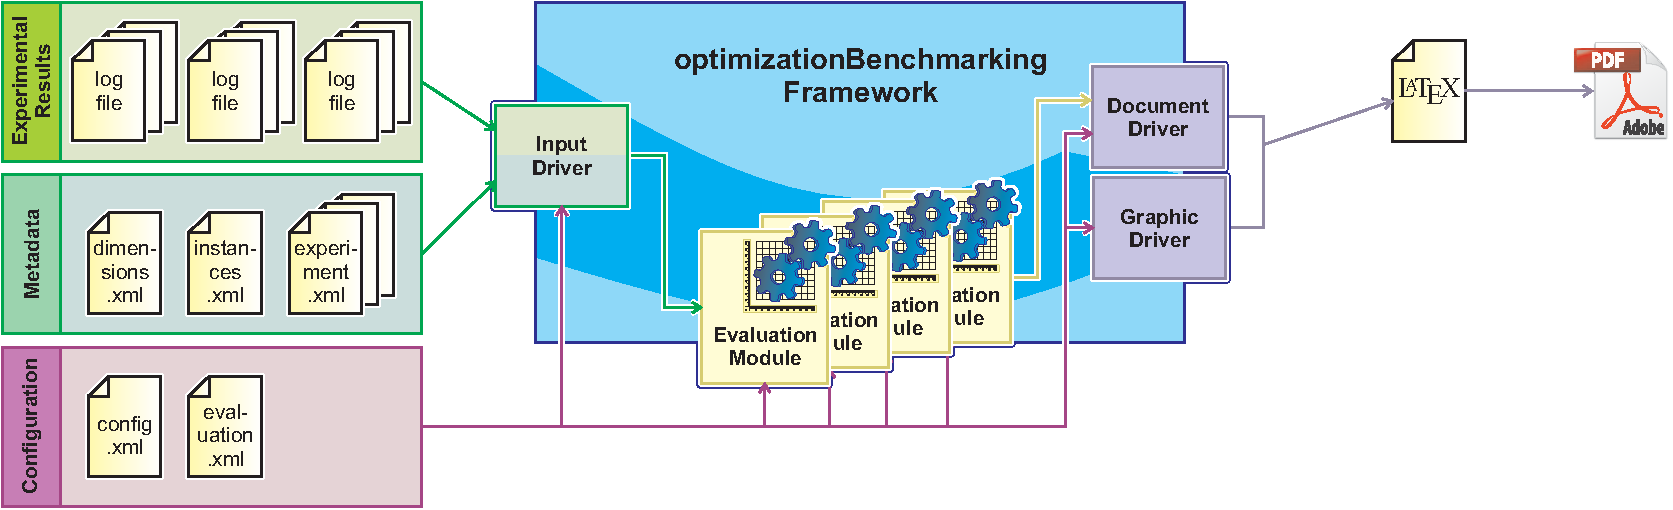
\includegraphics[width=0.9\paperwidth]{graphics/flow/flow_output_4_pdf}}{0.05}{0.16}%
\locate{21}{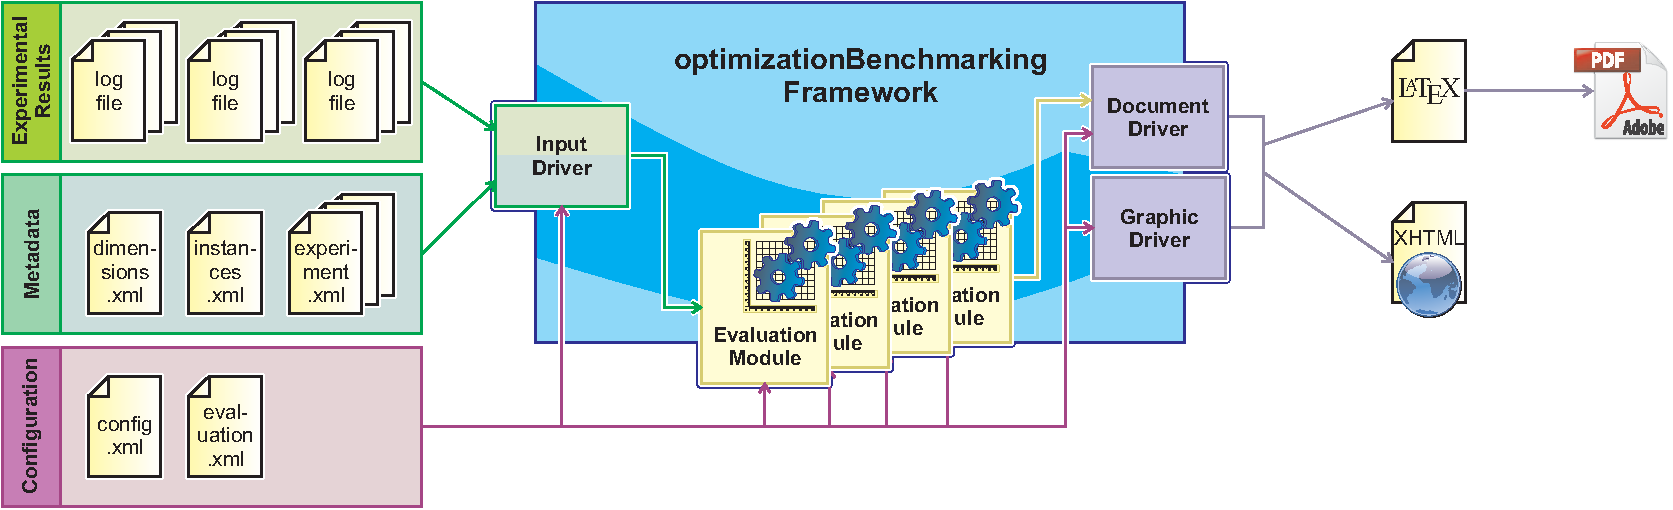
\includegraphics[width=0.9\paperwidth]{graphics/flow/flow_output_5_xhtml}}{0.05}{0.16}%
\locate{22-}{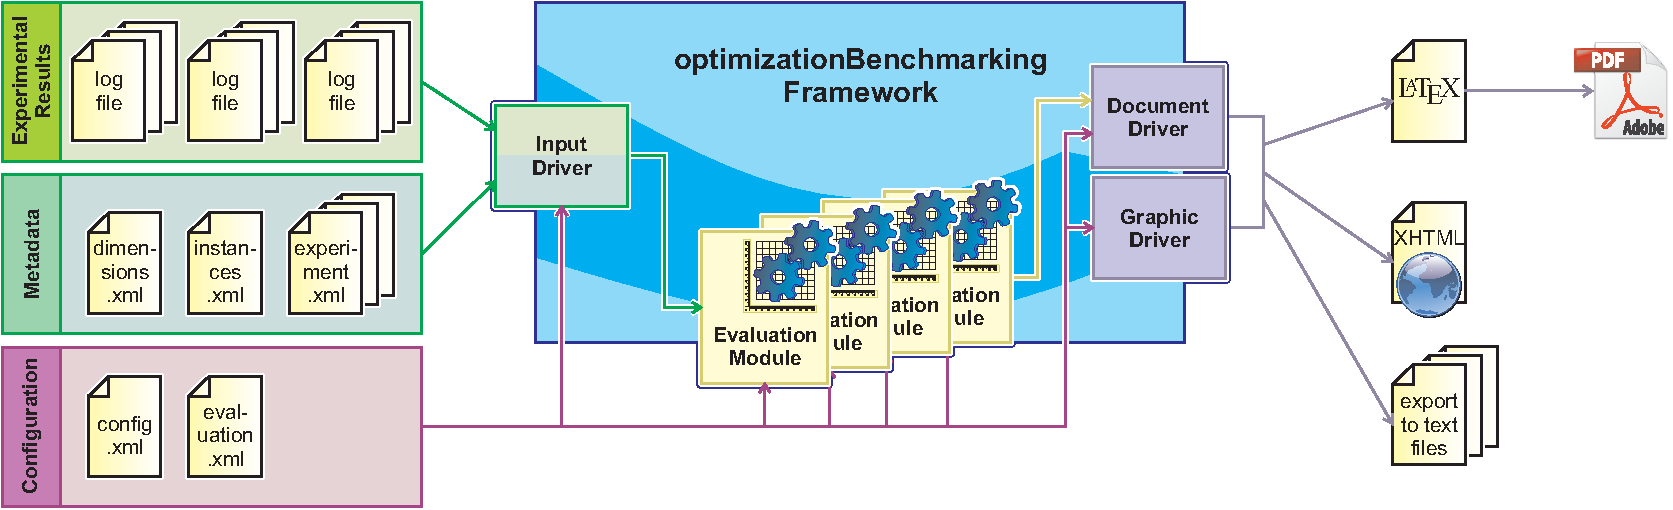
\includegraphics[width=0.9\paperwidth]{graphics/flow/flow}}{0.05}{0.16}%
%
\only<2->{%
\begin{small}%
\begin{itemize}%
%
\only<-9>{%
\item We got a couple of log files for each experiment\uncover<3->{: 6 experiments in our example, each with $10\times 10\times 20=\numprint{2000}$ log files}%
%}%
%
%\only<4-5>{%
\item<4-> We specify which dimensions we have measured\uncover<5->{: \measureFEs, \measureRuntime, and \measureObjectiveValue\ in our example\uncover<-5>{ (\alert{demo})}}%
%}%
%
%\only<6-7>{%
\item<6-> We specify which benchmark instances we have and what their features are\uncover<7->{: $10\times 10$ instances in our example, with features \maxSatVariables\ and \maxSatClauses\uncover<-7>{ (\alert{demo})}}%
%}%
%
%\only<8-9>{%
\item<8-> For each experiment, we specify the parameters\uncover<9->{: in our example, these are \texttt{algorithm}, \texttt{operator}, \texttt{restart}\uncover<-9>{ (\alert{demo})}}%
}%
%
\only<10-13>{%
\item<10-> An \inQuotes{input driver} loads the data\uncover<11->{: most commonly, the data will be in Comma-, Tab-, or Space-Separated-Values format (\textit{CSV}), but we also support \bbob\expandafter\scitep{\bbobReferences} and \tspSuite\expandafter\scitep{\tspSuiteReferences}}%
%}%
%
%\only<12>{%
\item<12-> Via a configuration file, we choose which input and output formats to use, as well as which file specifies the evaluation process%
%}%
%
%\only<13>{%
\item<13-> The \texttt{evaluation.xml} specifies \emph{how} to evaluate the data, i.e., which evaluation modules to apply%
}%
%
\only<14-15>{%
\item<14-> An evaluation module prints on particular type of information about an experiment or experiment set, such as the ECDF, or a table with final results, etc\dots%
\item<15-> Evaluation modules can be applied multiple times, with different configurations (e.g., we can plot ECDFs for different target solution qualities)%
}%
%
\only<16>{%
\item<16-> We can choose among several different formats to be used for graphics, including EPS\scitep{A1992EPFFS}, PDF\scitep{ISO320002008}, PGF (\LaTeX), SVG(Z), EMF, PNG\scitep{RFC2083}, GIF\scitep{CI1990GIFV8}, BMP, and JPG%
\\\strut%
\vspace{0.19\paperheight}%
\strut\\%
}%
%
%
\only<17->{%
\item<17-> We can also choose among different formats for the report documents, including\only<-17>{\dots}%
%
\uncover<18->{ %
\LaTeX\scitep{MGBCR2004TLC,GMS1994TLC,L1994LADPSUGARM,OPHS2011TNSSITLOLI1M}\only<21->{, XHTML\scitep{W3C2010XHTML,C2009NPOHXADHC}\only<22->{, and export to other programs}}\uncover<19-20>{:%
\begin{itemize}%
\item can automatically be compiled to PDF\scitep{ISO320002008}, if a \LaTeX\ compiler (such as TeXLive\scitep{TEXLIVE} or MiKTeX\scitep{MIKTEX}) is auto-detected%
\item<20-> different document classes, such as IEEEtran\scitep{IEEETRAN}, Springer LLNCS\scitep{SPRINGERLNCS}, ACM sig-alternate\scitep{ACMSIGALTERNATE} can be chosen%
\end{itemize}%
}}%
}%
%
\end{itemize}%
\end{small}}%
%
\end{frame}%
%
%